\documentclass[xetex,mathserif,serif]{beamer}
\usepackage{polyglossia}
\setdefaultlanguage[babelshorthands=true]{russian}
\usepackage{minted}
\usepackage{tabu}
\usepackage[11pt]{moresize}

\useoutertheme{infolines}

\usepackage{fontspec}
\setmainfont{FreeSans}
\newfontfamily{\russianfonttt}{FreeSans}

\usepackage{textpos}
\setlength{\TPHorizModule}{1cm}
\setlength{\TPVertModule}{1cm}

\definecolor{links}{HTML}{2A1B81}
\hypersetup{colorlinks,linkcolor=,urlcolor=links}

\tabulinesep=0.7mm

\title{Лекция 15: Основы сетевой безопасности}
\author[Юрий Литвинов]{Юрий Литвинов \newline \textcolor{gray}{\small\texttt{yurii.litvinov@gmail.com}}}

\newcommand{\attribution}[1] {
\vspace{-5mm}\begin{flushright}\begin{scriptsize}\textcolor{gray}{\textcopyright\, #1}\end{scriptsize}\end{flushright}
}

\date{16.05.2022}

\begin{document}

    \frame{\titlepage}

    \section{Введение}

    \begin{frame}
        \frametitle{Сетевая безопасность}
        \begin{itemize}
            \item Почти все сервисы требуют авторизации и обеспечения безопасности
            \item Аутентификация --- установление личности (точнее, идентичности) участника взаимодействия
            \begin{itemize}
                \item Обычно взаимна
            \end{itemize}
            \item Авторизация --- установление прав на выполнение операции
            \item Шифрование --- обеспечение конфиденциальности передаваемой информации
            \item Также важны:
            \begin{itemize}
                \item Целостность --- злоумышленник ничего не поменял
                \item Актуальность --- злоумышленник не проиграл старое сообщение
            \end{itemize} 
        \end{itemize}
    \end{frame}

    \begin{frame}
        \frametitle{Некоторые соображения}
        \begin{itemize}
            \item Основные уязвимости в современных системах не технические по характеру
            \item Большинство попыток взлома --- изнутри организации
            \item Сетевая безопасность --- игра против живого, умного и часто хорошо оснащённого противника
            \begin{itemize}
                \item Задача средств безопасности --- не сделать взлом невозможным, а сделать его нерентабельным
            \end{itemize}
            \item За протоколами безопасности стоит большая наука
            \begin{itemize}
                \item Придумать свой хитрый шифр или протокол аутентификации в общем случае очень плохая идея
            \end{itemize} 
            \item tradeoff между безопасностью и удобством использования
        \end{itemize}
    \end{frame}

    \section{Шифрование}

    \begin{frame}
        \frametitle{Шифрование}
        \begin{center}
            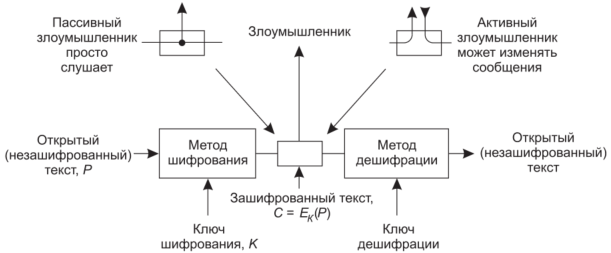
\includegraphics[width=0.6\textwidth]{cryptography.png}
            \attribution{Э. Таненбаум}
        \end{center}
        \begin{itemize}
            \item Алгоритм шифрования считается известным, секретен только ключ
            \item Усложнение алгоритма шифрования не всегда повышает криптостойкость
        \end{itemize}
        \begin{textblock}{2}(0,-6)
            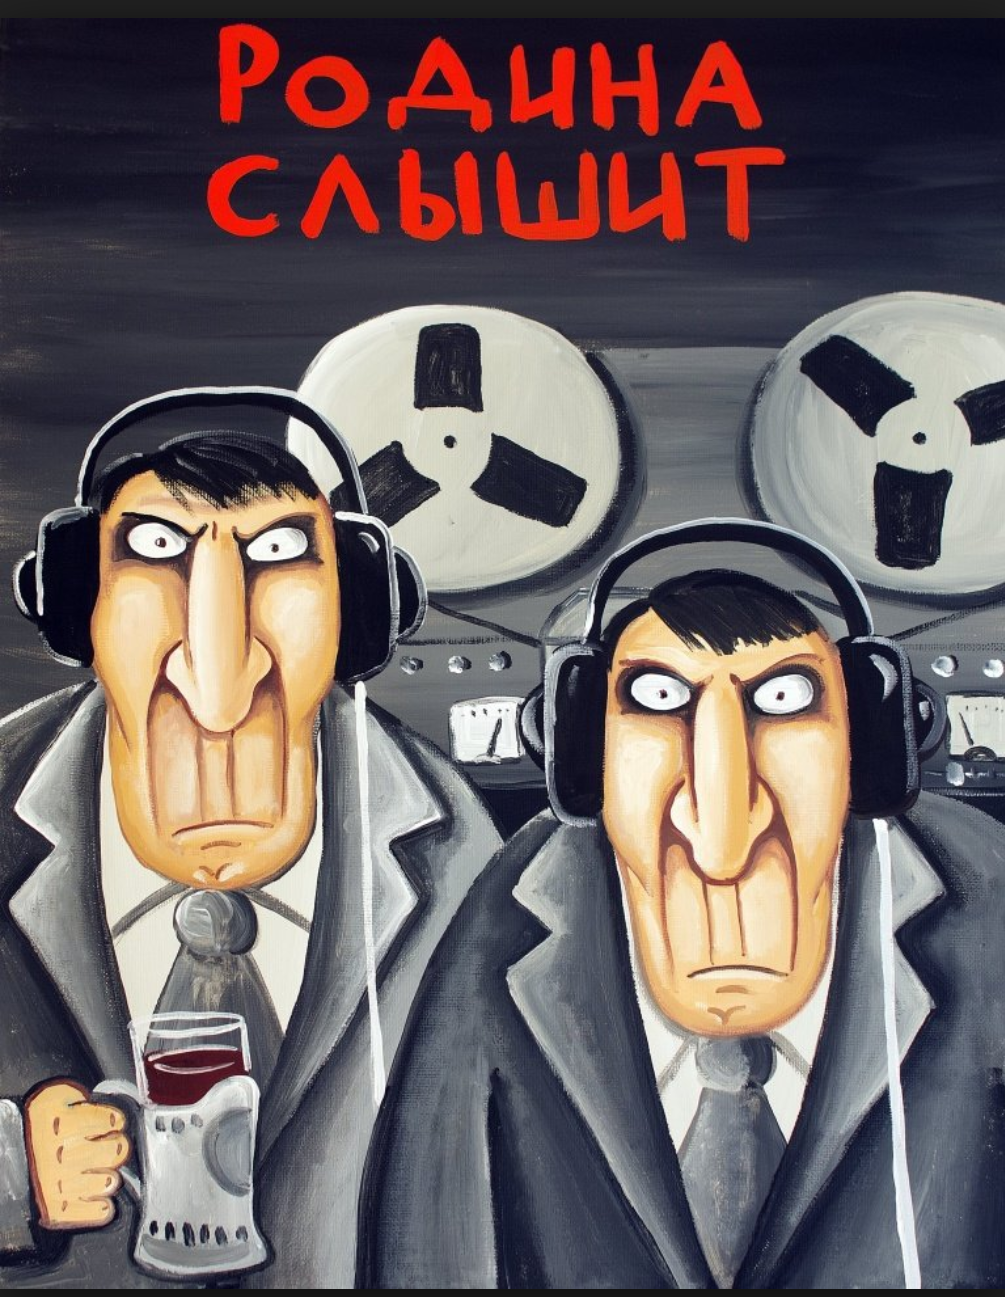
\includegraphics[width=\textwidth]{youAreBeingWatched.png}
        \end{textblock}
    \end{frame}

    \subsection{Шифрование с симметричным ключом}

    \begin{frame}
        \frametitle{Шифрование с симметричным ключом}
        \begin{itemize}
            \item Data Encryption Standard (DES, Triple DES)
            \item Advanced Encryption Standard (AES, он же Rijndael)
        \end{itemize}
        \begin{center}
            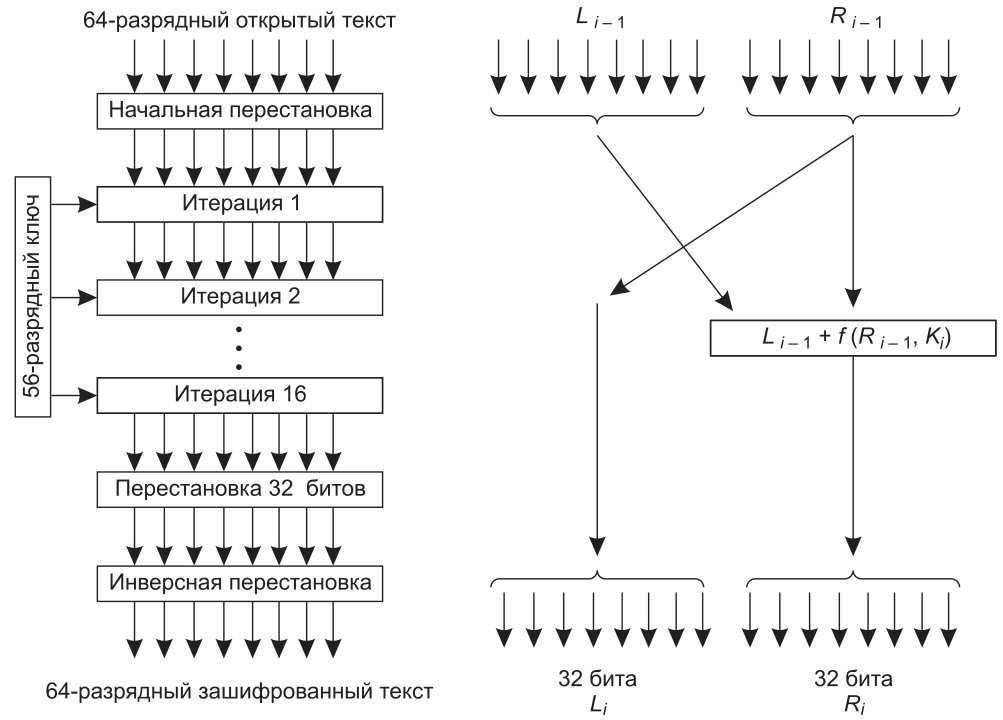
\includegraphics[width=0.6\textwidth]{des.png}
            \attribution{Э. Таненбаум}
        \end{center}
    \end{frame}

    \subsection{Режимы шифрования}

    \begin{frame}
        \frametitle{Режимы шифрования, ECB}
        \begin{itemize}
            \item Electronic Code Book --- один ключ применяется ко всем блокам
            \begin{itemize}
                \item Быстро, надёжно, но не криптостойко
            \end{itemize}
        \end{itemize}
        \begin{center}
            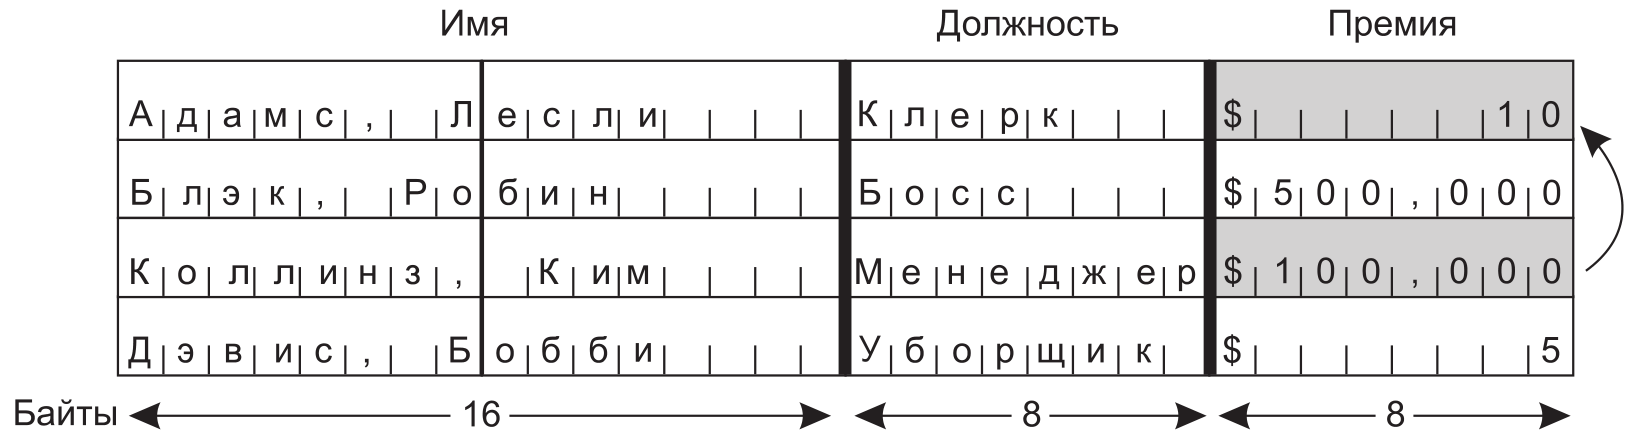
\includegraphics[width=0.85\textwidth]{ecbAttack.png}
            \attribution{Э. Таненбаум}
        \end{center}
    \end{frame}

    \begin{frame}
        \frametitle{Режимы шифрования, CBC}
        \begin{itemize}
            \item Cipher Block Chaining --- xor-им следующий блок с зашифрованным предыдущим перед шифровкой
            \begin{itemize}
                \item Более криптостоек, не устойчив к ошибкам передачи
                \item Initialization Vector (IV)
            \end{itemize}
        \end{itemize}
        \begin{center}
            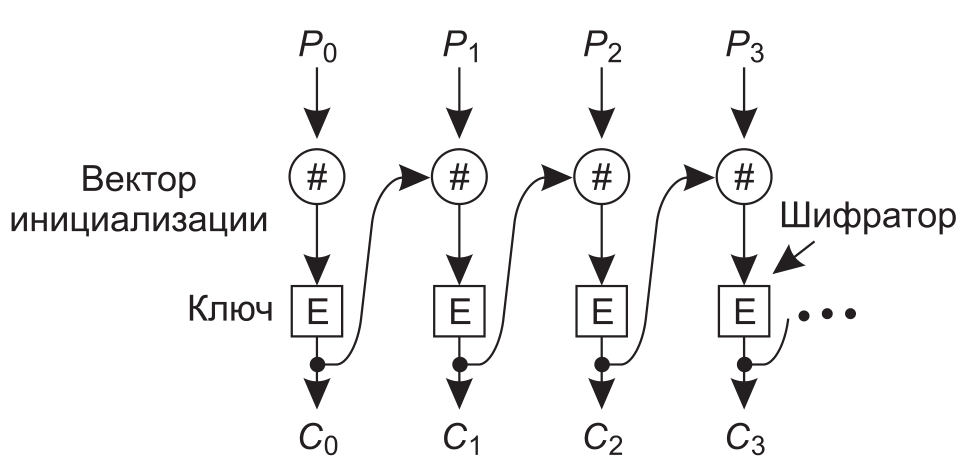
\includegraphics[width=0.6\textwidth]{cbc.png}
            \attribution{Э. Таненбаум}
        \end{center}
    \end{frame}

    \begin{frame}
        \frametitle{Режимы шифрования, SCM}
        \begin{itemize}
            \item Stream Cipher Mode --- шифруем IV ключом снова и снова, генерируя ключ бесконечной длины
            \begin{itemize}
                \item И xor-им его с шифруемым текстом
                \item Устойчив к ошибкам передачи, довольно быстр
                \item Уязвим к Keystream Reuse Attack ($(P_0 \oplus K_0) \oplus (Q_0 \oplus K_0)$)
            \end{itemize}
        \end{itemize}
        \begin{center}
            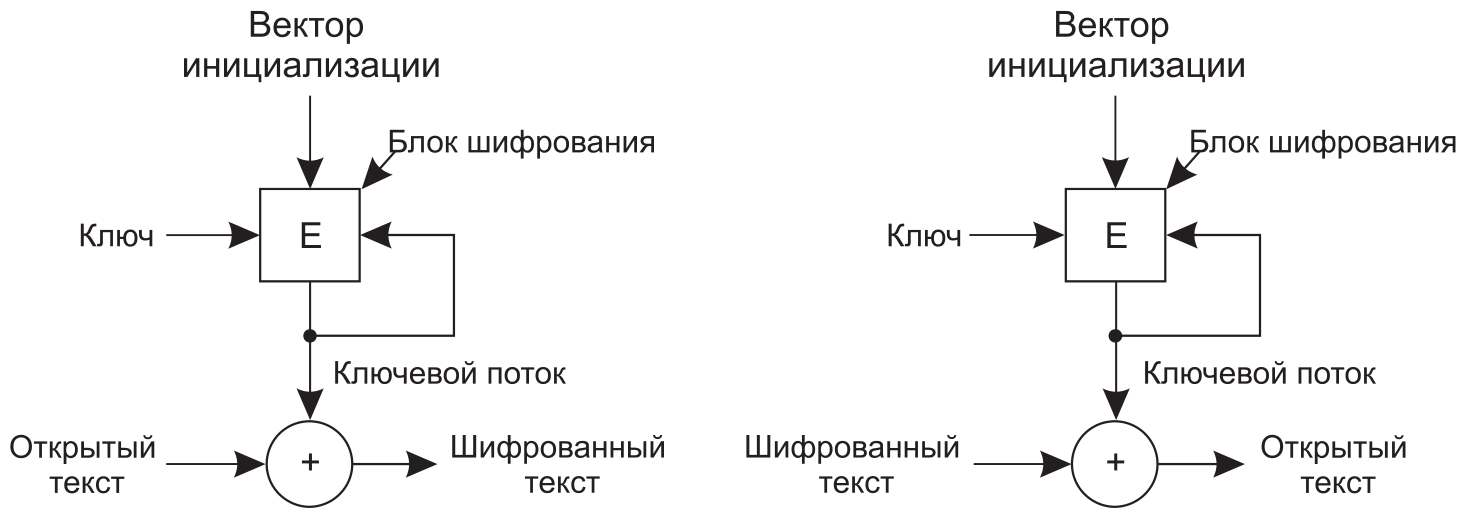
\includegraphics[width=0.85\textwidth]{scm.png}
            \attribution{Э. Таненбаум}
        \end{center}
    \end{frame}

    \begin{frame}
        \frametitle{Режимы шифрования, Counter Mode}
        \begin{itemize}
            \item Counter Mode --- шифруем $IV + i$ для каждого $i$-го блока
            \begin{itemize}
                \item И xor-им его с шифруемым текстом
                \item Для произвольного доступа к зашифрованным блокам
            \end{itemize}
        \end{itemize}
        \begin{center}
            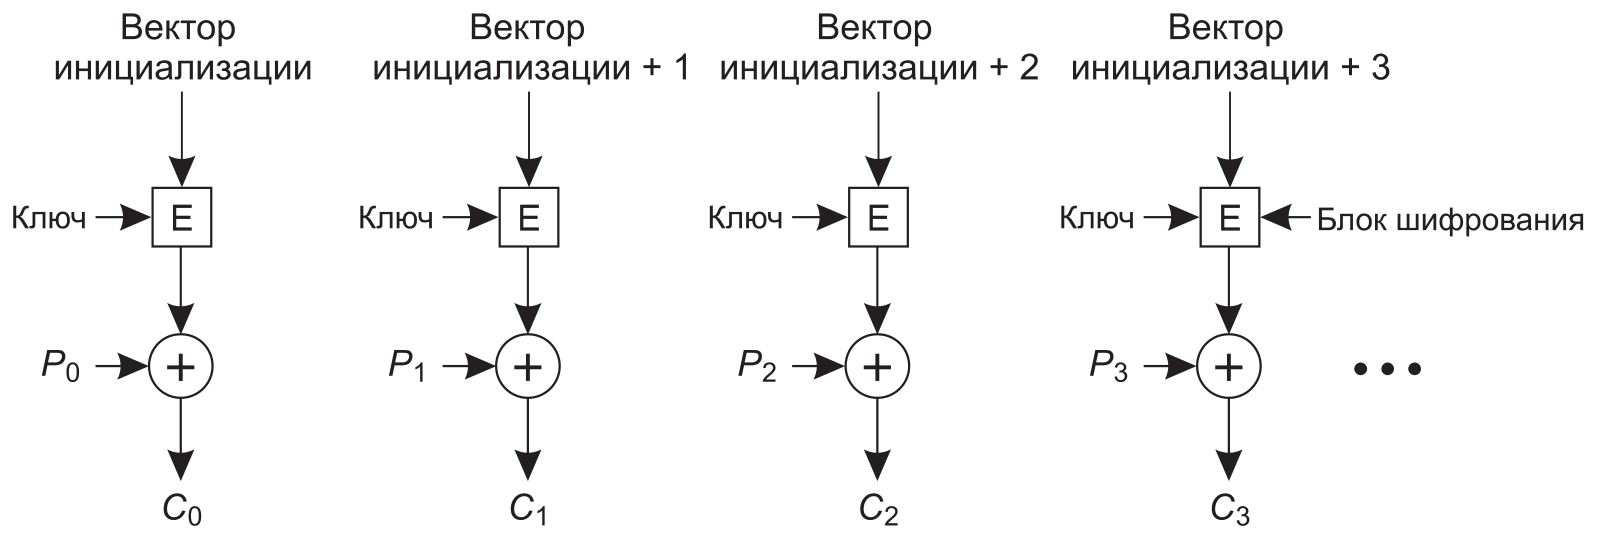
\includegraphics[width=0.85\textwidth]{cm.png}
            \attribution{Э. Таненбаум}
        \end{center}
    \end{frame}

    \subsection{Алгоритм Диффи-Хеллмана}

    \begin{frame}
        \frametitle{Алгоритм Диффи-Хеллмана}
        \begin{center}
            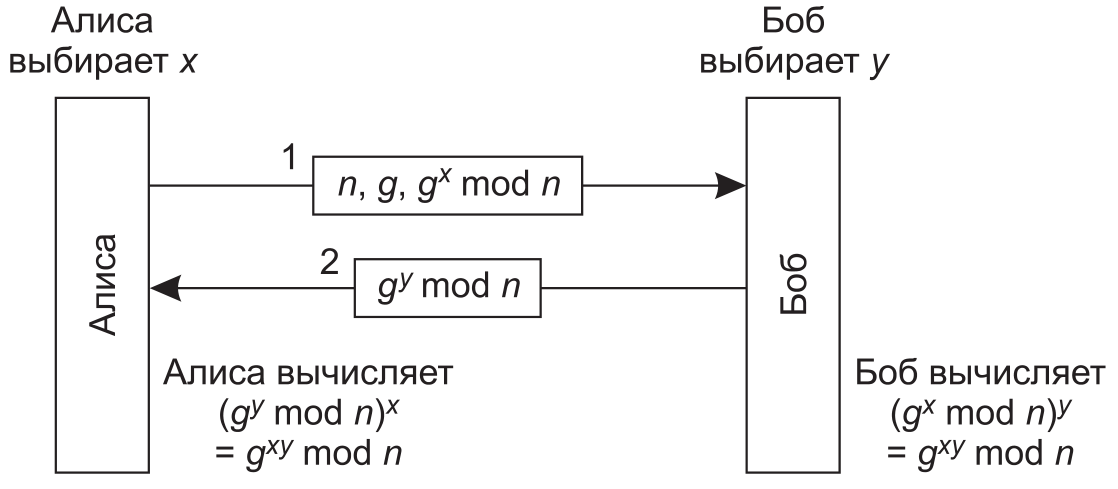
\includegraphics[width=0.6\textwidth]{diffieHellman.png}
            \attribution{Э. Таненбаум}
        \end{center}
    \end{frame}

    \begin{frame}
        \frametitle{Атака ``Man In The Middle''}
        \begin{center}
            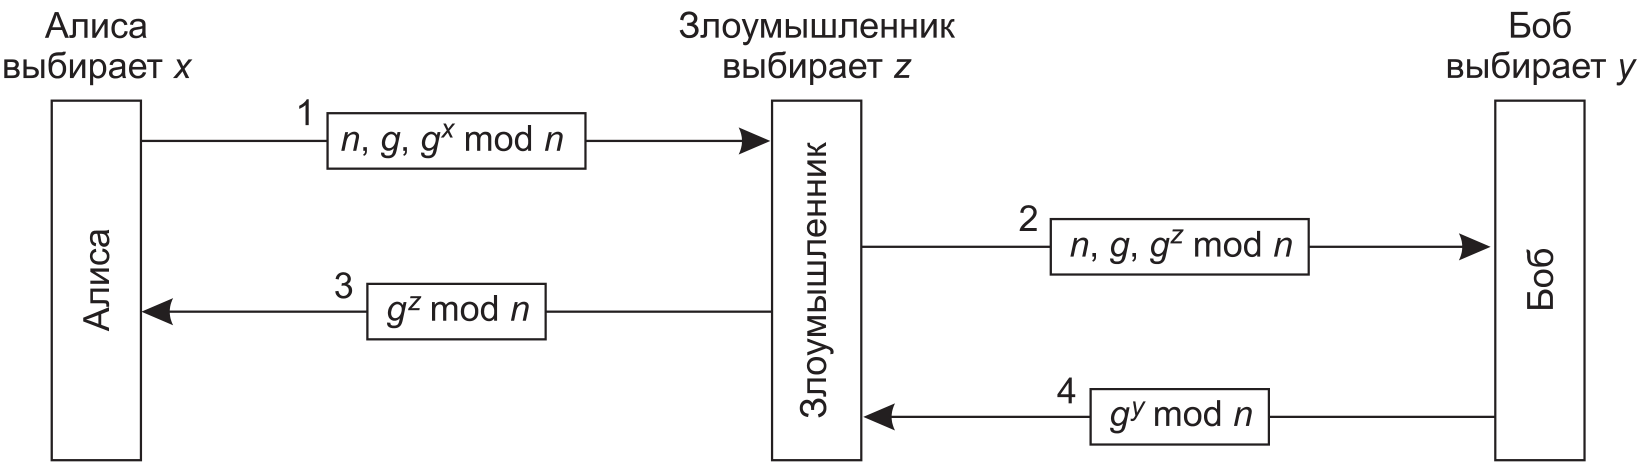
\includegraphics[width=0.9\textwidth]{diffieHellmanMitm.png}
            \attribution{Э. Таненбаум}
        \end{center}
    \end{frame}

    \subsection{Шифрование с открытым ключом}

    \begin{frame}
        \frametitle{Шифрование с открытым ключом}
        \framesubtitle{Или почему нельзя отдать ключи от Telegram}
        \begin{itemize}
            \item Алгоритм делится на две части, D и E, так, что D(E(P)) = P
            \item D очень сложно получить по E
            \begin{itemize}
                \item Например, найти простые сомножители огромного числа или дискретный логарифм по заданному модулю
            \end{itemize}
            \item E не ломается атакой ``произвольного открытого текста''
            \item D (ключ от D) держится в секрете, E выкладывается в открытый доступ
            \item Если Боб хочет послать Алисе сообщение, он берёт её открытый ключ $E_A$, шифрует им сообщение $P$ и отправляет Алисе
            \item Алиса дешифрует сообщение, вычисляя $D_A(E_A(P))$
            \item У каждого пользователя своя пара ключей
            \item Алгоритмы: RSA, ElGamal, эллиптические шифры
        \end{itemize}
    \end{frame}

    \section{Цифровые подписи}

    \begin{frame}
        \frametitle{Цифровые подписи, задачи}
        \begin{itemize}
            \item Получатель может установить личность отправителя
            \item Отправитель не может отрицать, что он подписал сообщение
            \item Получатель не может сам подделать сообщение и сделать вид, что его послал отправитель
        \end{itemize}
    \end{frame}

    \begin{frame}
        \frametitle{Цифровые подписи, реализация}
        \begin{center}
            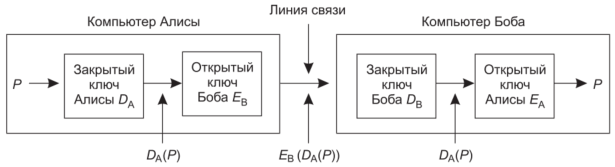
\includegraphics[width=0.7\textwidth]{signature.png}
            \attribution{Э. Таненбаум}
        \end{center}
        \begin{itemize}
            \item Надо, чтобы $D(E(P)) = P$ (это так для большинства криптосхем)
            \item Шифровать всё сообщение слишком медленно
            \item Message Digest-ы --- хорошие хеши сообщений
            \begin{itemize}
                \item MD5, SHA-1
            \end{itemize}
            \item Подписывается только хеш, это почти так же криптостойко, но в сотни раз быстрее
        \end{itemize}
    \end{frame}

    \begin{frame}
        \frametitle{SHA-1}
        \begin{itemize}
            \item Считается блоками по 512 бит, возвращает 160-битный дайджест
            \item Изменение в одном бите входа даёт совершенно другой выход
            \item Если известен $P$, очень сложно найти такой $P\ '$, что $MD(P\ ') = MD(P)$
        \end{itemize}
        \begin{center}
            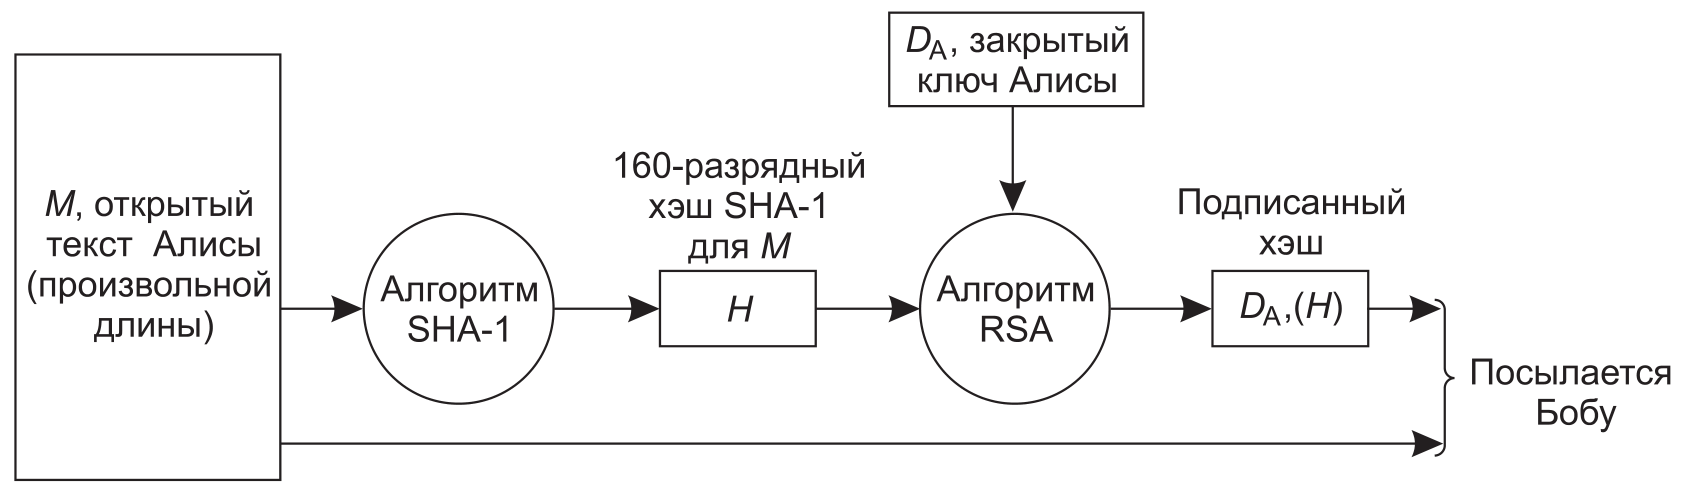
\includegraphics[width=0.85\textwidth]{sha1Signature.png}
            \attribution{Э. Таненбаум}
        \end{center}
    \end{frame}

    \begin{frame}
        \frametitle{Атака дней рождения}
        \begin{scriptsize}
Уважаемый господин декан,

\vspace{3mm}

Это [письмо | обращение] отражает мое [искреннее | откровенное] [мнение | суждение] о проф. Томе Уилсоне, являющемся [кандидатом | претендентом] на профессорскую должность в [настоящее время | этом году]. Я [знакома | работала] с проф. Уилсоном в течение [почти | около] шести лет. Он является [слабым | недостаточно талантливым] [исследователем | ученым], почти не известным в той области науки, которой он занимается. В его работах практически не заметно понимания [ключевых | главных] [проблем | вопросов] современности.

\vspace{3mm}

[Более | Кроме] того, он также не является сколько-нибудь [уважаемым | ценимым] [преподавателем | педагогом]. Его студенты дают его [занятиям | лекциям] [самые низкие | негативные] оценки. Он самый непопулярный [преподаватель | учитель] нашей кафедры, [славящийся | печально известный] своей [привычкой | склонностью] [высмеивать | ставить в неудобное положение] студентов, осмелившихся задавать вопросы на его [лекциях | занятиях].

\vspace{3mm}

% [Кроме | Помимо] того, [гранты | контракты] проф. Уилсона [почти | практически] не пополняют [фондов | финансовых запасов] нашей кафедры. Если не удастся быстро найти новый источник финансирования, [мы будем вынуждены | нам придется] [закрыть | прекратить] [много | ряд] [важных | специальных] программ, [таких как | среди которых] государственная программа 2000 года. К сожалению, при таких [условиях | обстоятельствах] я не могу [предлагать | рекомендовать] его вам на эту должность.
        \end{scriptsize}
    \end{frame}

    \section{Сертификаты}

    \begin{frame}
        \frametitle{Сертификаты}
        \begin{center}
            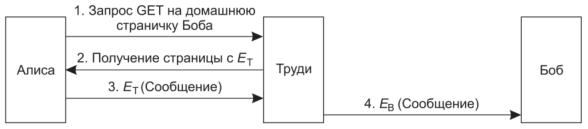
\includegraphics[width=0.6\textwidth]{manInTheMiddle.png}
            \attribution{Э. Таненбаум}
        \end{center}
        \begin{itemize}
            \item Сертификат --- сообщение, подтверждающее идентичность ключа, подписанное Certificate Authority (стандарт X.509)
            \item Цепочка сертификатов --- CA верхнего уровня подписывает сертификаты CA уровнем ниже, чтобы они могли подписывать сертификаты пользователей
            \item Корневые сертификаты --- сертификаты, которым принято доверять
            \item Самоподписанные сертификаты --- не доверенные, используются для отладки
        \end{itemize}
    \end{frame}

    \begin{frame}
        \frametitle{Сертификаты (2)}
        \begin{center}
            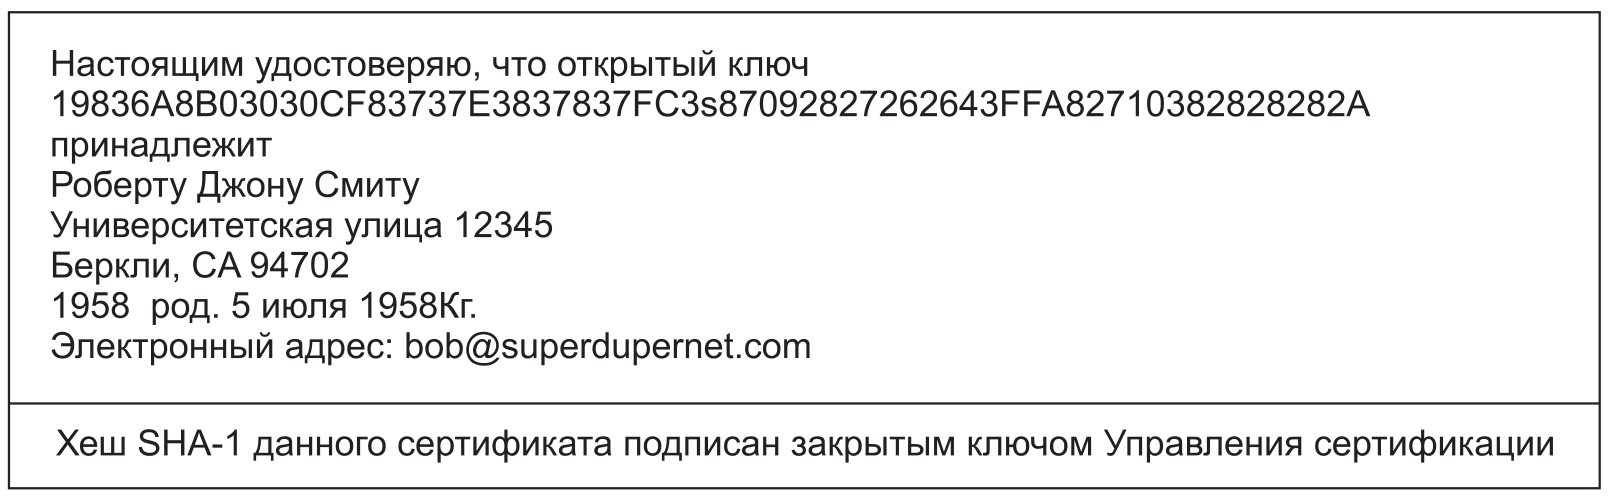
\includegraphics[width=0.65\textwidth]{certificate.png}
            \attribution{Э. Таненбаум}
        \end{center}
        \begin{itemize}
            \item Подписанный у CA сертификат стоит денег (от \$7 до более \$200 в год, в зависимости от типа)
            \begin{itemize}
                \item И требует идентификации личности (например, по паспорту)
                \item Есть бесплатно и без бюрократии, но ими далеко не всё можно подписать
            \end{itemize}
            \item Сертификаты всегда выдаются на фиксированное время
            \item Сертификат можно отозвать
            \item Куча несовместимых форматов: .pem, .p12, .pfx, .der, .cer, .crt
        \end{itemize}
    \end{frame}

    \begin{frame}
        \frametitle{Certificate Authority}
        \begin{center}
            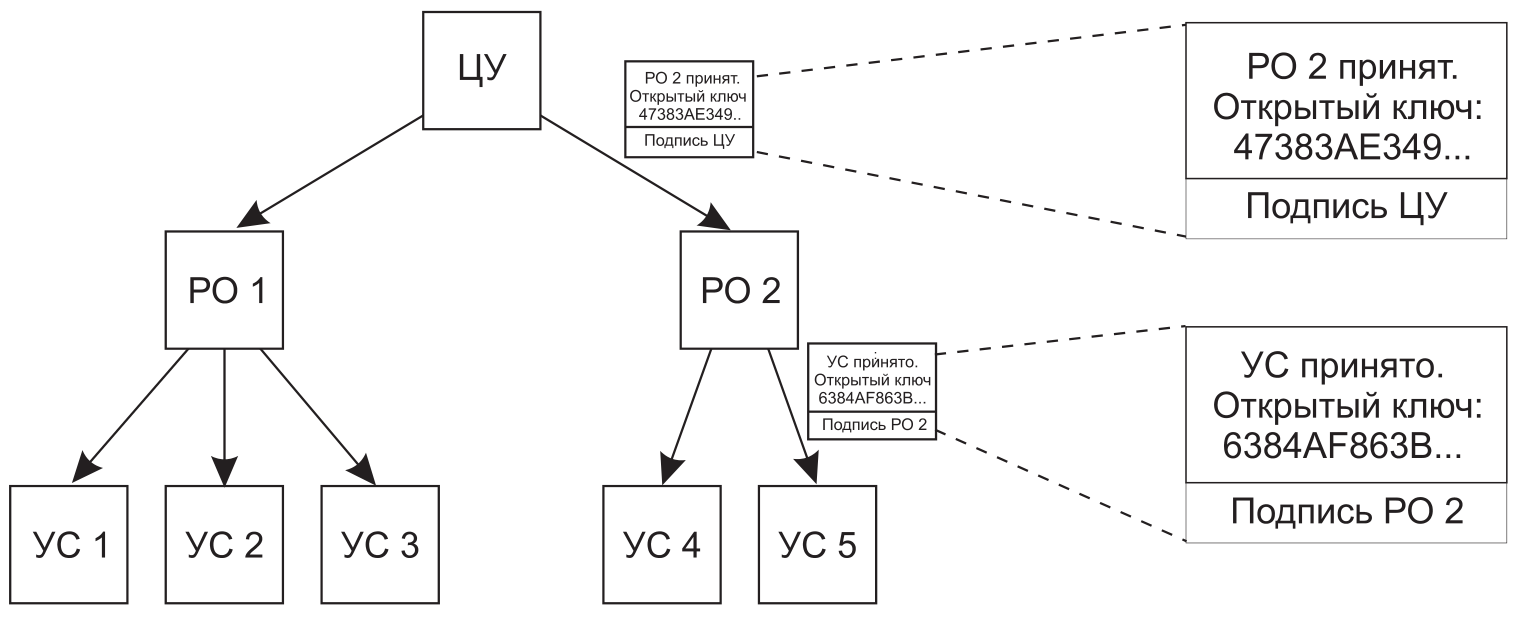
\includegraphics[width=0.85\textwidth]{certHierarchy.png}
            \attribution{Э. Таненбаум}
        \end{center}
        \begin{itemize}
            \item \url{https://letsencrypt.org/} --- автоматически и бесплатно даёт сертификаты, но они подтверждают только владение доменом, а не личность хозяина
        \end{itemize}
    \end{frame}

    \begin{frame}
        \frametitle{Применения сертификатов}
        \begin{itemize}
            \item Протокол HTTPS, проверка идентичности сервера
            \item Подписывание кода (Windows SmartScreen, Apple Code Signing)
            \item Подписывание сборок, сильные имена сборок в .NET
        \end{itemize}
        \begin{center}
            \includegraphics[width=0.6\textwidth]{dotNetCodeSigning.png}
            \attribution{J. Richter}
        \end{center}
    \end{frame}

    \begin{frame}
        \frametitle{Менеджер сертификатов, Windows}
        \framesubtitle{Snap-In в MMC}
        \begin{center}
            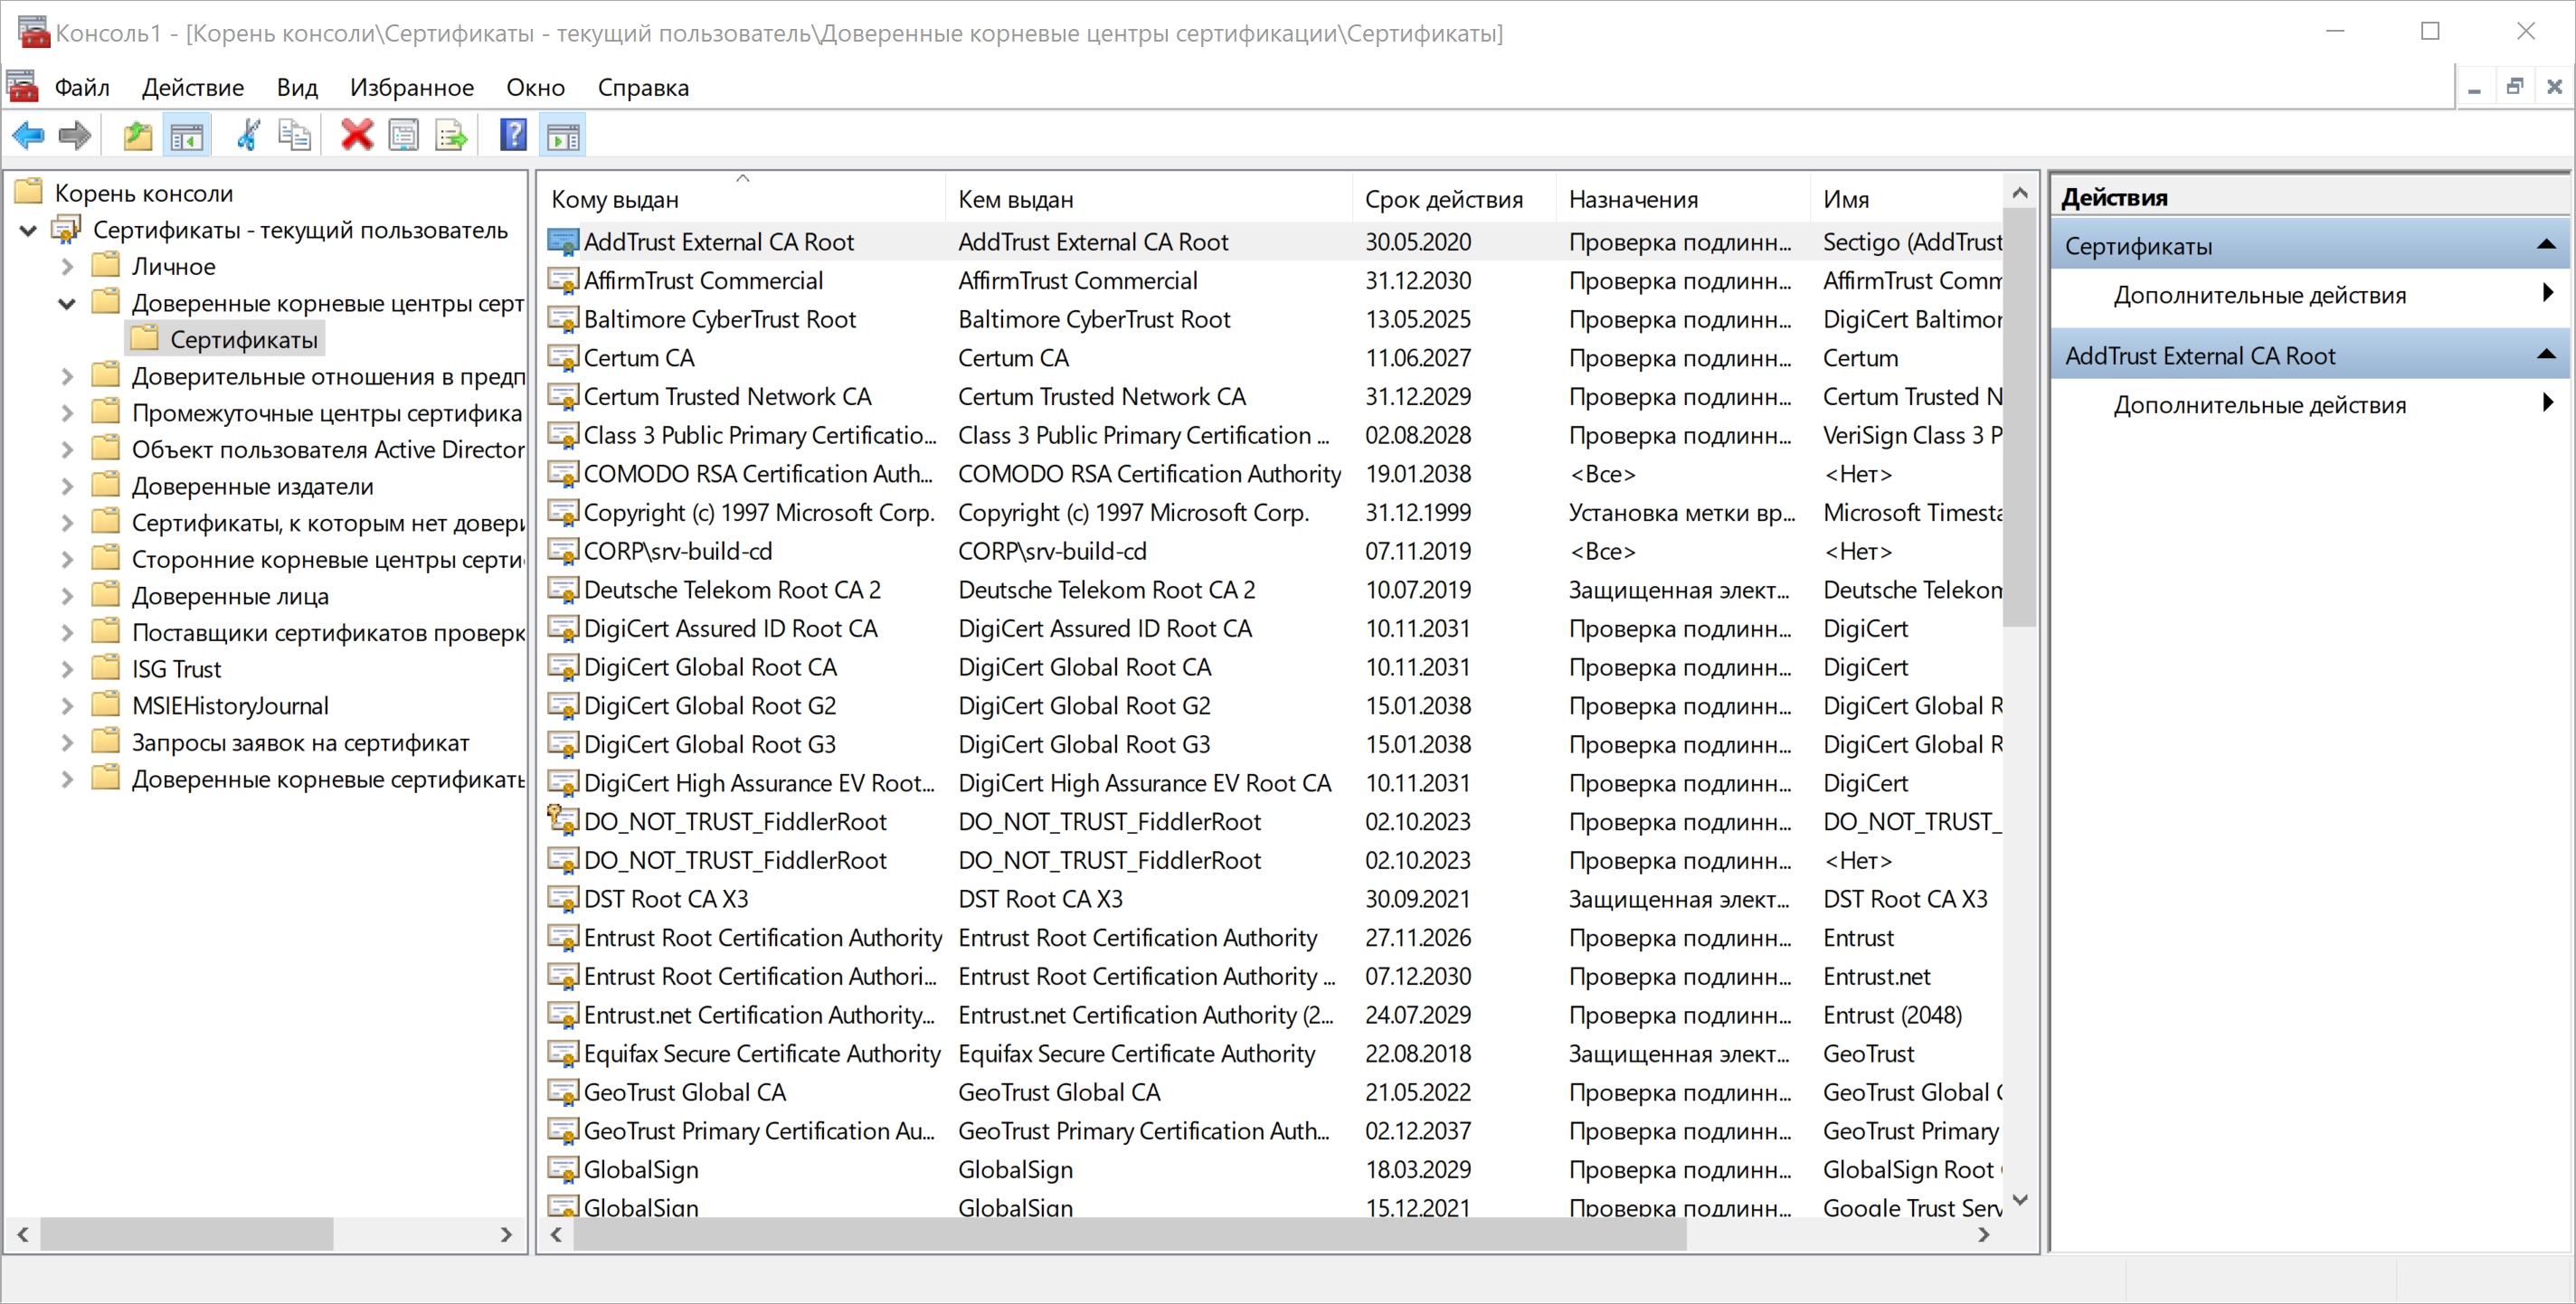
\includegraphics[width=0.95\textwidth]{windowsCertManager.png}
        \end{center}
    \end{frame}

    \begin{frame}[fragile]
        \frametitle{OpenSSL}
        \begin{itemize}
            \item OpenSSL --- библиотека и набор инструментов для криптографии и работы с протоколами SSL/TLS
            \item Стандарт де-факто для работы с открытыми ключами, сертификатами и т.д.
            \item Как сгенерить самоподписанный сертификат:
            
                \begin{minted}{bash}
openssl req -x509 -nodes -days 365 
    -newkey rsa:2048 -keyout privatekey.key 
    -out certificate.crt
                \end{minted}
        \end{itemize}
    \end{frame}

    \section{Аутентификация}

    \subsection{Общий ключ}

    \begin{frame}
        \frametitle{Аутентификация Challenge-Response с общим ключом}
        \begin{center}
            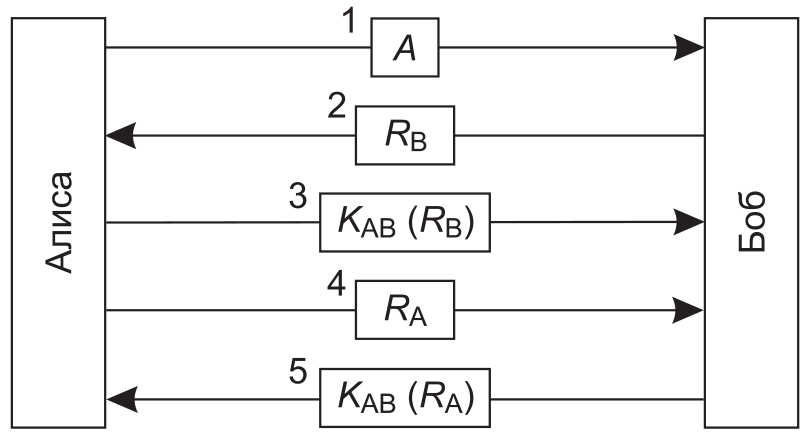
\includegraphics[width=0.5\textwidth]{challengeResponse.png}
            \attribution{Э. Таненбаум}
        \end{center}
        \begin{itemize}
            \item $R_B$ --- \textbf{nonce} (number used once), для предотвращения атаки повтором
            \item $K_{AB}$ --- общий ключ
        \end{itemize}
    \end{frame}

    \begin{frame}
        \frametitle{``Упрощённый'' протокол}
        \begin{center}
            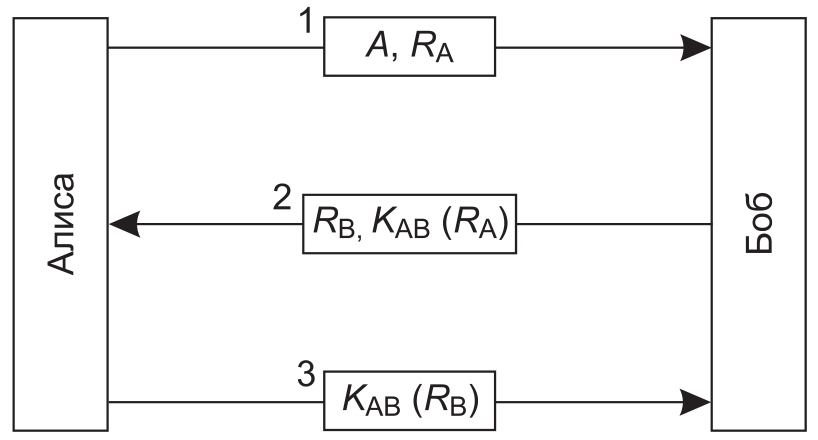
\includegraphics[width=0.5\textwidth]{simpleChallengeResponse.png}
            \attribution{Э. Таненбаум}
        \end{center}
    \end{frame}

    \begin{frame}
        \frametitle{Зеркальная атака}
        \begin{center}
            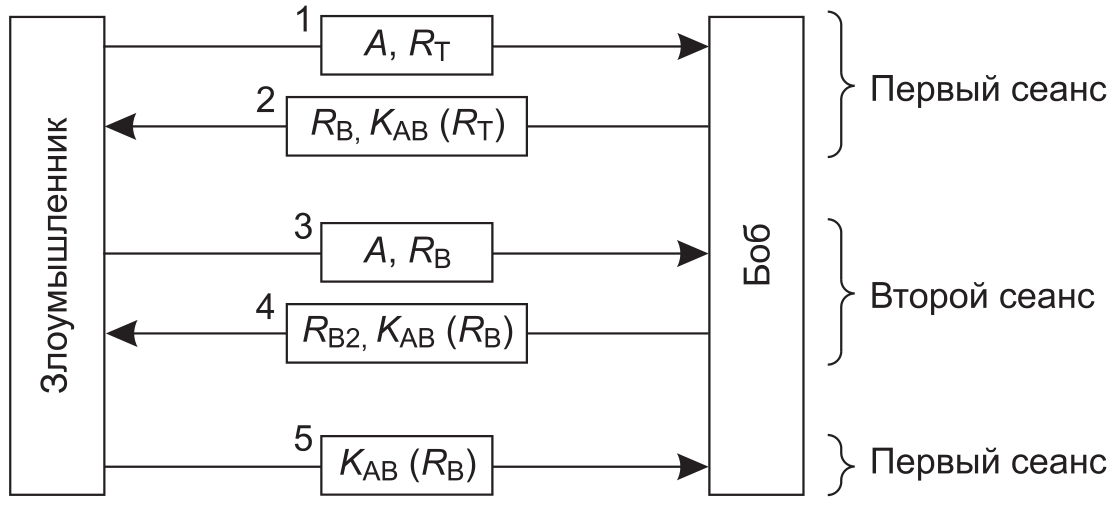
\includegraphics[width=0.65\textwidth]{mirrorAttack.png}
            \attribution{Э. Таненбаум}
        \end{center}
        \vspace{5mm}
        \textbf{Разработать корректный протокол аутентификации сложнее, чем это может показаться}
    \end{frame}

    \begin{frame}
        \frametitle{Правильный протокол}
        \begin{center}
            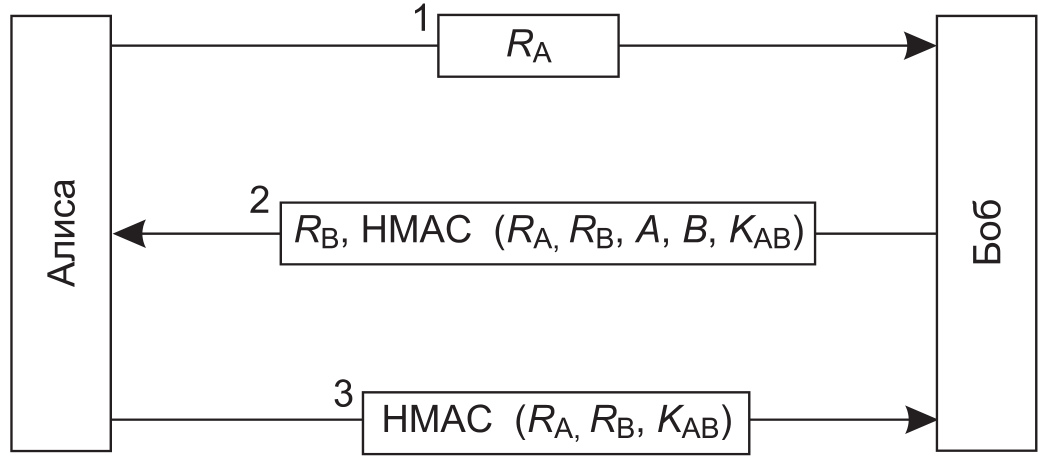
\includegraphics[width=0.6\textwidth]{hmacs.png}
            \attribution{Э. Таненбаум}
        \end{center}
        \begin{itemize}
            \item HMAC --- Hashed Message Authentication Code
        \end{itemize}
    \end{frame}

    \begin{frame}
        \frametitle{Как на самом деле}
        \begin{itemize}
            \item Basic Authentication --- логин и пароль передаются нешифрованными в заголовке HTTP-запроса
            \item HTTPS обеспечивает безопасность
            \item Сервер возвращает Access Token
            \item Access Token предъявляется при каждом следующем запросе
            \begin{itemize}
                \item Имеет ограниченное время жизни, но его можно продлять
            \end{itemize}
            \item Пароли не хранятся на сервере, хранятся их хеши
            \begin{itemize}
                \item Salt --- случайное число, дописываемое к паролю на стороне сервера, хранится вместе с хешем пароля
                \item Если базу паролей украдут, узнать исходные пароли очень сложно
            \end{itemize}
        \end{itemize}
    \end{frame}

    \begin{frame}
        \frametitle{Аутентификация с открытым ключом}
        \begin{center}
            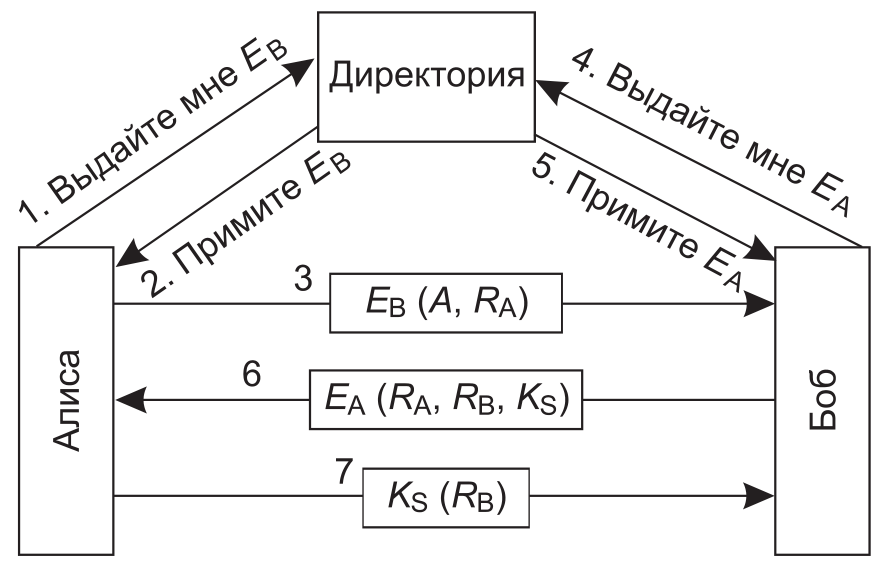
\includegraphics[width=0.6\textwidth]{openKeyAuthentication.png}
            \attribution{Э. Таненбаум}
        \end{center}
        \begin{itemize}
            \item $E_A$, $E_B$ --- открытые ключи Алисы и Боба
            \item $R_A$, $R_B$ --- nonce
        \end{itemize}
    \end{frame}

    \subsection{OAuth2}

    \begin{frame}
        \frametitle{OAuth 2}
        \begin{itemize}
            \item Позволяет разрешить пользование ресурсом, не раскрывая хозяину ресурса логин и пароль пользователя
            \begin{itemize}
                \item Логин по аккаунту в Google или аккаунту в VK
            \end{itemize}
            \item Роли:
            \begin{itemize}
                \item Client --- приложение, пытающееся получить доступ
                \item Resource Server --- сервер, хранящий защищённую информацию. К нему пытается получить доступ клиент
                \item Resource Owner --- пользователь, владеющий защищённой информацией
                \item Authorization Server --- сервер, выдающий клиенту токен на доступ к ресурсному серверу
            \end{itemize}
        \end{itemize}
    \end{frame}

    \begin{frame}
        \frametitle{Протокол}
        \begin{center}
            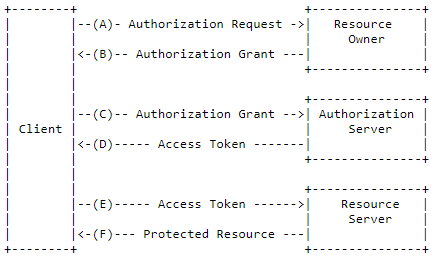
\includegraphics[width=0.5\textwidth]{oauth.png}
            \attribution{RFC 6749}
        \end{center}
    \end{frame}

    \begin{frame}
        \frametitle{Детали}
        \begin{itemize}
            \item Access Token --- выдаётся авторизационным сервером и посылается с каждым запросом, ограниченное время жизни
            \item Refresh Token --- выдаётся авторизационным сервером, используется для получения нового Access Token
            \item Scope --- к какой части ресурса даёт доступ Access Token
        \end{itemize}
    \end{frame}

    \begin{frame}
        \frametitle{Пример: Google OAuth 2.0}
        \begin{columns}
            \begin{column}{0.5\textwidth}
                \begin{itemize}
                    \item Google Developer Console, Client ID и Client Secret
                    \item Scope
                    \item Consent Screen
                \end{itemize}
            \end{column}
            \begin{column}{0.4\textwidth}
                \begin{center}
                    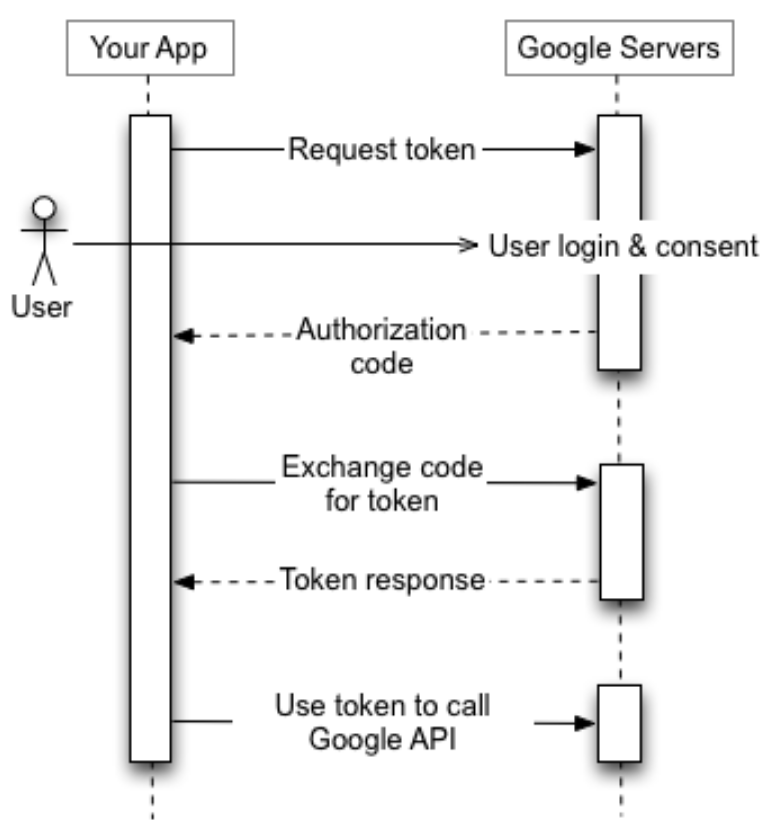
\includegraphics[width=\textwidth]{googleOAuth.png}
                    \attribution{\url{https://developers.google.com}}
                \end{center}
            \end{column}
        \end{columns}
    \end{frame}

    \section{Безопасность транспортного уровня}

    \begin{frame}
        \frametitle{HTTPS}
        \begin{center}
            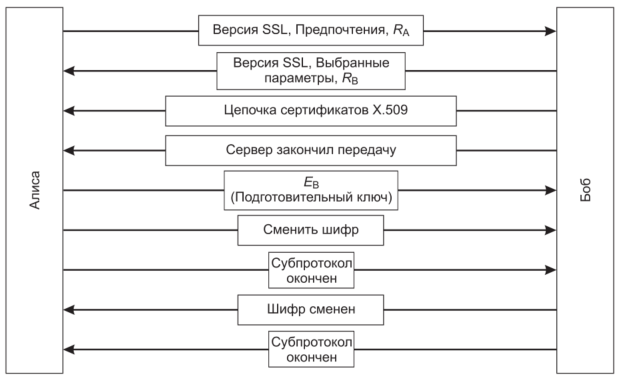
\includegraphics[width=0.6\textwidth]{ssl.png}
            \attribution{Э. Таненбаум}
        \end{center}
        \begin{itemize}
            \item SSL (Secure Sockets Layer)
            \item HTTPS --- HTTP через SSL
            \item Порт 443
            \item Аутентифицируется только сервер
        \end{itemize}
    \end{frame}

    \begin{frame}
        \frametitle{SSL, транспортный субпротокол}
        \begin{center}
            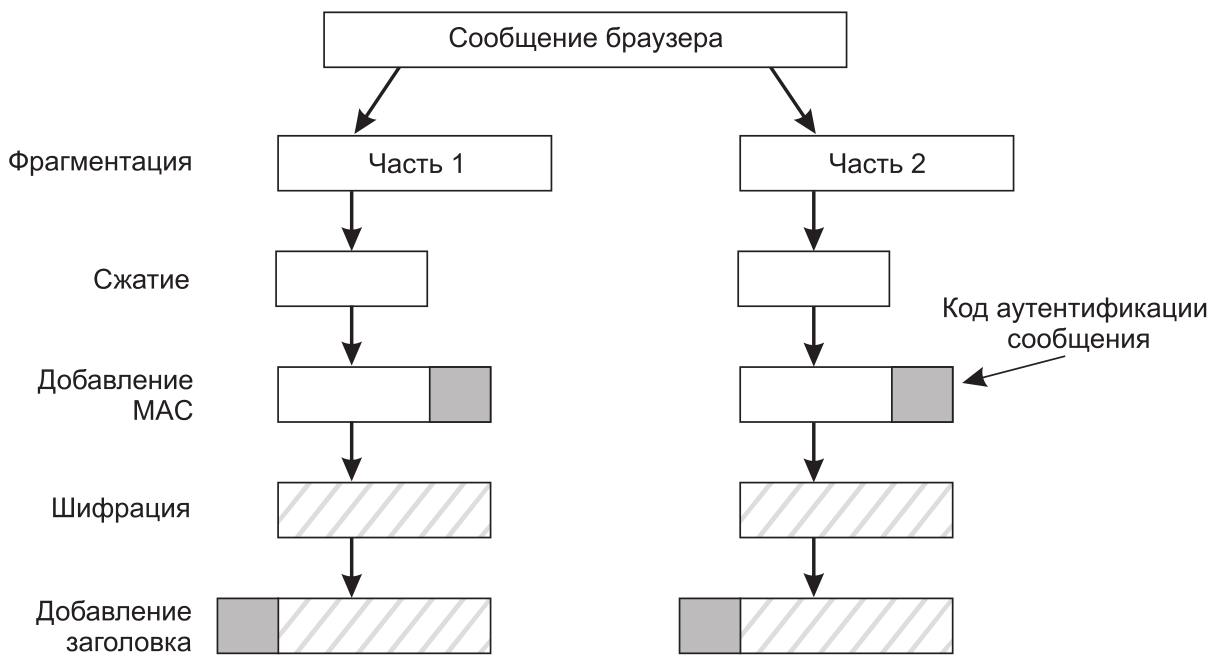
\includegraphics[width=0.6\textwidth]{sslCommunication.png}
            \attribution{Э. Таненбаум}
        \end{center}
        \begin{itemize}
            \item Triple DES + SHA-1
            \item Или RC4 со 128-битным ключом + MD5
            \item TLS --- Transport Layer Security (продвинутый SSL)
        \end{itemize}
    \end{frame}

    \begin{frame}
        \frametitle{DNS Spoofing}
        \begin{columns}
            \begin{column}{0.4\textwidth}
                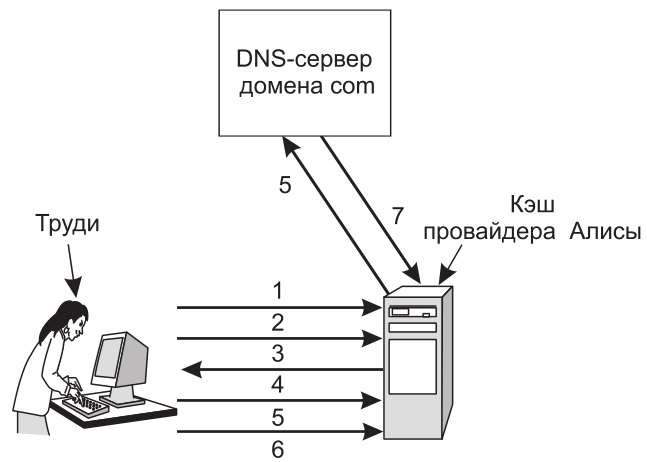
\includegraphics[width=0.95\textwidth]{dnsSpoofing.png}
                \attribution{Э. Таненбаум}
            \end{column}
            \begin{column}{0.6\textwidth}
                \begin{footnotesize}
                    \begin{enumerate}
                        \item Запрос foobar.trudy-the-intruder.com (чтобы trudy-the-intruder.com попал в кеш провайдера)
                        \item Запрос www.trudy-the-intruder.com (чтобы получить следующий порядковый номер провайдера)
                        \item Запрос об адресе www.trudy-the-intruder.com к нашему DNS
                        \item Запрос к bob.com
                        \item Запрос о bob.com к DNS зоны com
                        \item Подделанный ответ о bob.com
                        \item Настоящий ответ, отвергнутый, потому что уже поздно
                    \end{enumerate}
                \end{footnotesize}
            \end{column}
        \end{columns}
    \end{frame}

    \begin{frame}
        \frametitle{Результат}
        \begin{center}
            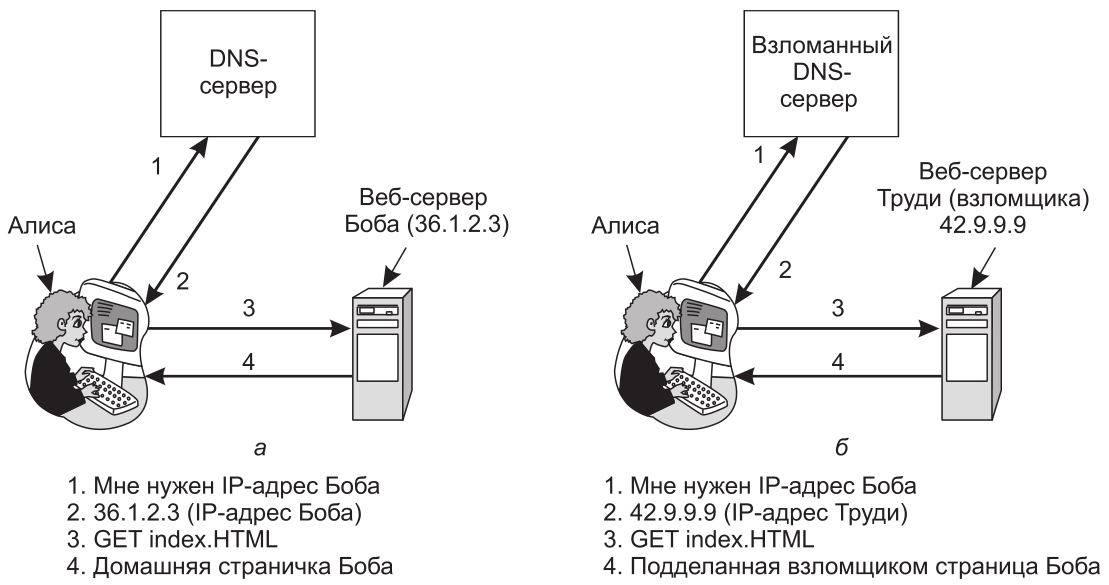
\includegraphics[width=0.9\textwidth]{dnsSpoofingResult.png}
            \attribution{Э. Таненбаум}
        \end{center}
    \end{frame}

    \section{Отладка}

    \begin{frame}
        \frametitle{Как это всё отлаживать}
        \framesubtitle{И ломать}
        \begin{itemize}
            \item Fiddler --- кроссплатформенный отладочный прокси
            \begin{itemize}
                \item Перехват HTTP-трафика
                \item Man-In-The-Middle-атака с самоподписанными сертификатами
                \begin{itemize}
                    \item Расшифровка HTTPS-трафика на лету
                \end{itemize}
                \item Возможность модифицировать HTTP-пакеты, повторять пакеты и т.д.
            \end{itemize}
            \item Wireshark --- когда Fiddler-а мало
            \begin{itemize}
                \item Перехват пакетов на низком уровне
                \item Умеет даже ставить себя как драйвер USB и читать USB-пакеты
            \end{itemize}
        \end{itemize}
    \end{frame}

\end{document}